\section{Softwarearchitektur und Design}

\section*{5 Vorlesung 05}
\subsection*{5.1 Ubersicht Business Analyse vs Architektur vs Entwicklung}
\begin{center}
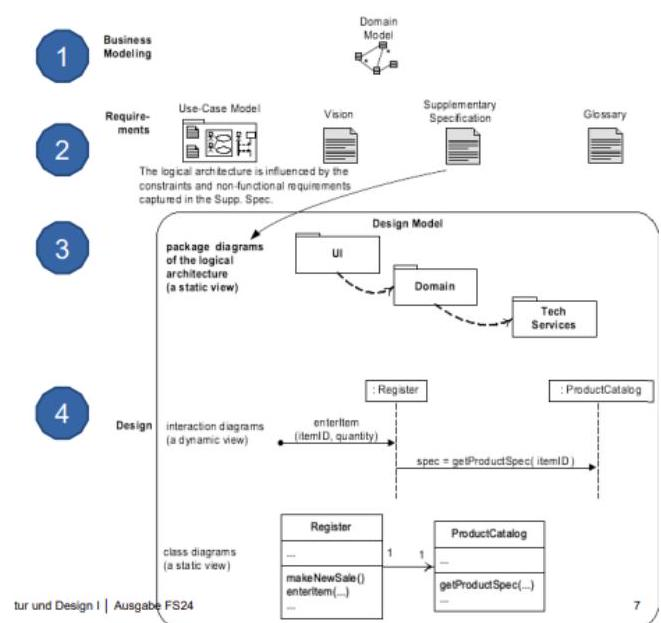
\includegraphics[width=\linewidth]{images/2024_12_29_0d1d7b5551ea1b4b41bdg-07(2)}
\end{center}

Abbildung 14: Übersicht Business Analyse vs Architektur vs Entwicklung

\begin{enumerate}
  \item Domänenmodell (Business Modelling) Kontext Diagramm (Business Analyst)
  \item Requirement (Business Analyst)
  \item Logische Architektur (Software Architekt)
  \item Umsetzung (Entwicklung)\\
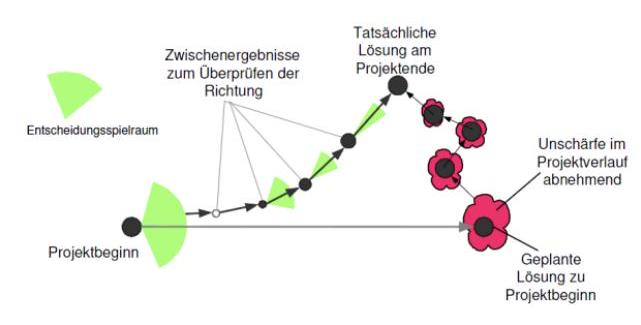
\includegraphics[width=\linewidth]{images/2024_12_29_0d1d7b5551ea1b4b41bdg-08(1)}
\end{enumerate}

Abbildung 15: Entstehung Archtektur

\subsection*{5.2 Architektur aus Anforderungen}
Die Architektur muss heutige und zukünftige Anforderungen erfüllen können und Weiterentwicklungen der Software und seiner Umgebung ermöglichen

\subsection*{5.2.1 Architekturanalyse}
Analyse der funktionalen und nichtfunktionalen Anforderungen:\\
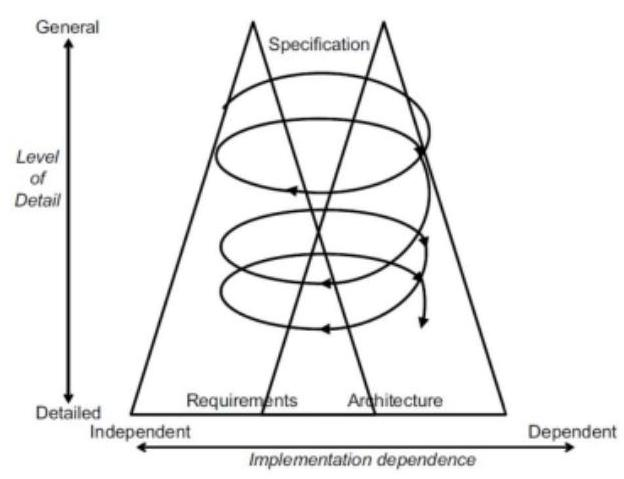
\includegraphics[width=\linewidth]{images/2024_12_29_0d1d7b5551ea1b4b41bdg-08}

Abbildung 16: Twin Peak Model\\
Entwurfsentscheidungen sollten in erster Linie aus den Anforderungen abgeleitet werden, Architekturentscheidungen und die Konsequenzen daraus müssen mit den Stakeholdern abgestimmt werden.

\subsection*{5.2.2 ISO 25010}
\begin{itemize}
  \item ISO 25010 provides a hierarchical structure for non-functional requirements.
  \item It defines main characteristics, sub-characteristics, and metrics.
  \item Each non-functional requirement in ISO 25010 is associated with metrics.
  \item Metrics include a description of the requirement, a measurement method to check requirement fulfillment, and guidance for interpreting results.
  \item This allows for more precise and measurable formulation of requirements, which can be verified later.\\
5.2.3 Difference from FURPS + (Functionality, Usiability, Reliability, Performance, Supportability (Anpassungsfähigkeit, Wartbarkeit, etc), $+=$ Implementation, Interface, Operations, Packaging, Legal)
  \item FURPS+ is an acronym and not a standard.
  \item FURPS+ includes Functionality, Usability, Reliability, Performance, Supportability, and other terms.
\end{itemize}

\subsection*{5.2.4 Grundprinzip: Modulkonzept}
Modul (Baustein, Komponente): Güte wird gemessen mit Kohäsion und Kopplung

\begin{itemize}
  \item Möglichst autarkes Teilsystem (wenig Kopplung nach aussen)
  \item Hat eine klare minimale Schnittstelle gegen aussen
  \item Software-Modul enthält alle Funktionen und Datenstrukturen, die es benötigt
  \item Modul kann sein: Paket, Programmierkonstrukt, Library, Komponente, Service
\end{itemize}

\subsection*{5.2.5 Architektur beschreiben}
Architektur umfasst verschiedene Aspekte, die je nach Sichtweise wichtig sind

\section*{N+1 View Model + 1 View: Use Cases}
\begin{center}
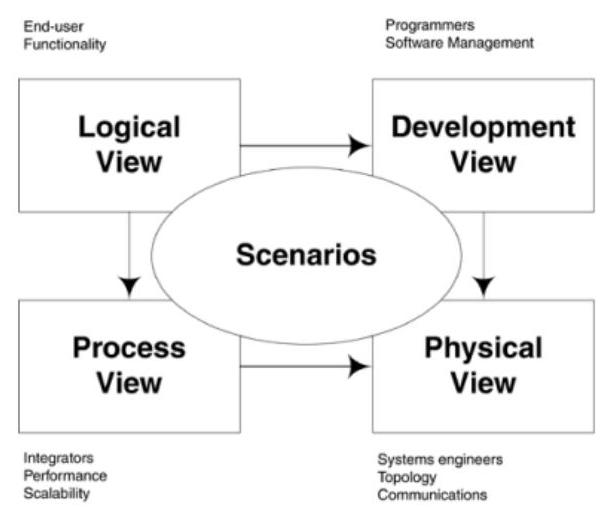
\includegraphics[width=\linewidth]{images/2024_12_29_0d1d7b5551ea1b4b41bdg-09}
\end{center}

Abbildung 17: View Model\\
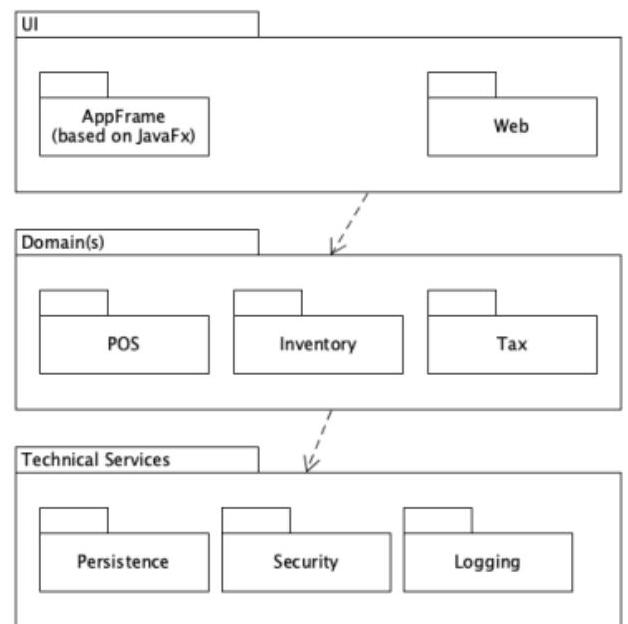
\includegraphics[width=\linewidth]{images/2024_12_29_0d1d7b5551ea1b4b41bdg-09(1)}

Abbildung 18: UML- Paketdiagram

\begin{itemize}
  \item Mittel, um Teilsysteme zu definieren
  \item Mittel zur Gruppierung von Elementen
\end{itemize}

Paket enthält Klassen und andere Pakete

\begin{itemize}
  \item Ähnlich, aber allgemeiner als Java Packages
\end{itemize}

Abhängigkeiten zwischen Paketen\\
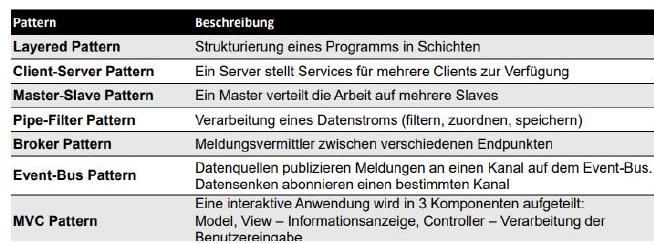
\includegraphics[width=\linewidth]{images/2024_12_29_0d1d7b5551ea1b4b41bdg-09(2)}

Abbildung 19: Architekturpatterns

\section*{6 Vorlesung 06}
\subsection*{6.1 Zweck und Anwendung von Statischen und Dynamischen Modellen im Design}
\begin{itemize}
  \item Statische Modelle, wie beispielsweise das UML-Klassendiagramm, unterstützen den Entwurf von Paketen, Klassennamen, Attributen und Methodensignaturen (ohne Methodenkörper).
  \item Dynamische Modelle, wie beispielsweise UMLInteraktionsdiagramme, unterstützten den Entwurf der Logik, des Verhaltens des Codes und der Methodenkörper.
\end{itemize}

Statische u Dynamische ergänzen sich, werden parallel erstellt

\subsection*{6.2 Objektentwurf mit UML-Klassen-, UML-Interaktions-, UML-Zustands- und UML-Aktivitätsdiagrammen}
\subsection*{6.2.1 UML-Klassendiagramm}
Notationselemente:

\begin{itemize}
  \item Klasse, aktive Klasse
  \item Attribut
  \item Operation
  \item Sichtbarkeit von Attributen und Operationen
  \item Assoziationsname, Rollen an den Assoziationsenden
  \item Multiplizität (Bezieht sich auf die Objekte der betreffenden Klasse)
  \item Navigierbarkeit in Assoziationen
  \item Datentypen und Enumerationen
  \item Generalisierung / Spezialisierung
  \item Abstrakte Klassen
  \item Assoziation, Assoziationsklasse: Komposition, Aggregation
  \item Interface, Interface Realisierung
\end{itemize}

\subsection*{6.2.2 UML-Interkationsdiagramm}
Modellieren die Kollaborationen bzw. den Informationsaustausch zwischen Objekten (Dynamik).

Sequenzdiagramm Notationselemente:

\begin{itemize}
  \item Lebenslinie
  \item Aktionssequenz
  \item Synchrone Nachricht
  \item Antwortnachricht
  \item Gefundene, verlorene Nachricht
  \item Kombiniertes Fragment
  \item Erzeugungs-, Löschereignis
  \item Selbstaufruf
  \item Interaktionsreferenz
  \item Lebensline mit aktiver Klasse
  \item Asynchrone Nachricht
\end{itemize}

\section*{Kommuninaktionsdiagramm}
\begin{itemize}
  \item Lebenslinie (Box)
  \item Synchrone Nachricht (= Aufruf einer Operation) (Nummeriert)
  \item Antwortnachricht (= Rückgabewert)
  \item Bedingte Nachrichten «[]»
  \item Iteration «*»
\end{itemize}

\subsection*{6.2.3 UML-Zustandsdiagramm}
Welche Zustände kann ein Objekt, eine Schnittstelle, ein Use Case, ... bei welchen Ereignissen annehmen?

\begin{itemize}
  \item Start-, Endzustand
  \item einfacher Zustand
  \item Zusammengesetzter bzw. geschachtelter Zustand
  \item Flache und tiefe Historie
  \item Transition
  \item Orthogonaler Zustand
  \item Parallelisierungsknoten
  \item Synchronisationsknoten
  \item Einstiegpunkt
  \item Ausstiegspunkt
  \item Unterzustandsautomat
\end{itemize}

\subsection*{6.2.4 UML-Aktivitätsdiagramm}
Wie läuft ein bestimmter Prozess oder ein Algorithmus ab?

\begin{itemize}
  \item Aktivität
  \item Aktionsknoten (Aktion)
  \item Objektknoten (Objekt)
  \item Entscheidungs- und Vereinigungsknoten
  \item Kante
  \item Initialknoten
  \item Aktivitätsendknoten
  \item Partition (auch Swimlane genannt)
  \item Parallelisierungsknoten
  \item Synchronisationsknoten
  \item SendSignal-Aktion
  \item Ereignis- bzw. Zeitereignisannahmeaktion
  \item CallBehavior-Aktion
\end{itemize}

\subsection*{6.3 Responsibility Driven Design (RDD)}
Denken in Verantwortlichkeiten, Rollen und Kollaborationsbeziehungen für den Entwurf von Softwareklassen.\\
RDD kann auf jeder Ebene des Designs angewendet werden (Klasse, Komponente, Schicht).\\
Verantwortlichkeiten werden durch Attribute und Methoden implementiert.

\subsection*{6.4 Prinizpien für Klassenentwurf: GRASP, SOLID}
\subsection*{6.4.1 SOLID: Missing from Slides}
6.4.2 GRASP (General Responsibility Assignment Software Patterns)

\begin{itemize}
  \item welche Klassen und Objekte wofür zuständig
  \item für erleichterung Kommunikation d Entwickler
  \item grundlegenden Prinzipen bzw. Pattern
  \item Information Expert: Ein Objekt sollte die Verantwortung für eine Aufgabe übernehmen, wenn es die benötigten Informationen dazu besitzt.
  \item Creator: Ein Objekt sollte für die Erstellung von anderen Objekten verantwortlich sein, wenn eine starke Beziehung zwischen ihnen besteht.
  \item Controller: Ein Objekt sollte die zentrale Steuerungslogik in einem System repräsentieren.
  \item Low Coupling: Objekte sollten lose miteinander gekoppelt sein, um die Flexibilität und Wiederverwendbarkeit des Systems zu erhöhen.
  \item High Cohesion: Eine Klasse sollte nur zusammengehörige Funktionen und Daten enthalten, um ihre Verständlichkeit und Wartbarkeit zu verbessern.
  \item Polymorphism: Objekte sollten so entworfen werden, dass sie anhand ihrer Schnittstellen verwendet werden können, unabhängig von ihrer spezifischen Implementierung.
  \item Pure Fabrication: Künstliche Klassen sollten erstellt werden, um eine hohe Kohäsion und niedrige Kopplung zu erreichen, wenn keine natürliche Klasse die Verantwortung übernehmen kann.
  \item Indirection: Zwischen Objekten sollten indirekte Verbindungen hergestellt werden, um die Flexibilität und Wartbarkeit zu erhöhen.
  \item Protected Variations: Mechanismen sollten eingeführt werden, um Variationen in den Systemkomponenten zu schützen und unerwünschte Auswirkungen von Änderungen zu minimieren.
\end{itemize}